\documentclass[main.tex]{subfiles}

\section{The Test Problem and DOPRI54}

In this first section we are going to implement a set of numerical methods for solving ordinary differential equations. Since the algorithms are only approximations to the real solution, we shall also test their accuracy and discuss their performance by comparing the results obtained when solving the two following initial value problems:

\begin{equation}
\dot{x} = \lambda x(t) \qquad
x(0) = 1 \qquad
\lambda = -1
\label{eq:TestEquation}
\end{equation}

\begin{equation}
\ddot{x} = -x(t) \qquad
x(0) = 1 \qquad
\dot{x}(0) = 0
\label{eq:HarmonicOscillator}
\end{equation}


\subsection{One step methods}

As a first approach, we will apply Explicit Euler's method. This basic algorithm makes use of finite difference methods to replace the derivatives in the differential equation. 

Considering a differential equation of the form:

\begin{equation}
\frac{dy}{dt} = f(t_n,y_n) \qquad
y(t_0) = y_0
\label{eq:ExplicitEuler}
\end{equation}

If the independent variable is discretized, the solution can be obtained in $n$ steps, by performing cosequtive approximations to the real function values.

\begin{equation}
y_{n+1} = y_{n} + h f(t_n,y_n)
\label{eq:ExplicitEuler}
\end{equation}

Where $h$ is then the size of the step. It is easy to show that the smaller the step size is the more accurate our solution will be.

Instead of using the previous iterate one could also look at future values to approximate a solution. This method is called backward or implicit Euler:

\begin{equation}
y_{n+1} = y_{n} + h f(t_{n+1},y_{n+1})
\label{eq:ExplicitEuler}
\end{equation}

However, for nonlinear problems the solution of the previous equation may require the use of numerical solvers, such as Newton's method, and thus the algorithm becomes computationally more demanding than the explicit Euler's method. We shall see in the next section the advantange of using this method.

Finally, the trapezodial method can be seen as a combination of both methods, where the solution is computed in every iteration by taking the average of the forward and backward finite difference approximations.

\begin{equation}
y_{n+1} = y_{n} + \frac{1}{2} h (f(t_{n+1},y_{n+1})
\label{eq:Trapezoidal}
\end{equation}

As in the previous case, \ref{eq:Trapezoidal} is an implicit equation and thus it might require the use of Newton's method to find a solution.
 
Figure \ref{fig:sol1} shows the solution from $t = 0$ to $t = 10$ of the two initial value problems given by explicit, implicit Euler and trapezoidal, along with the true solution. The solution is approximated in both cases by using  
30 points ($h = 0.345$).

\begin{figure}[H]
    \centering
    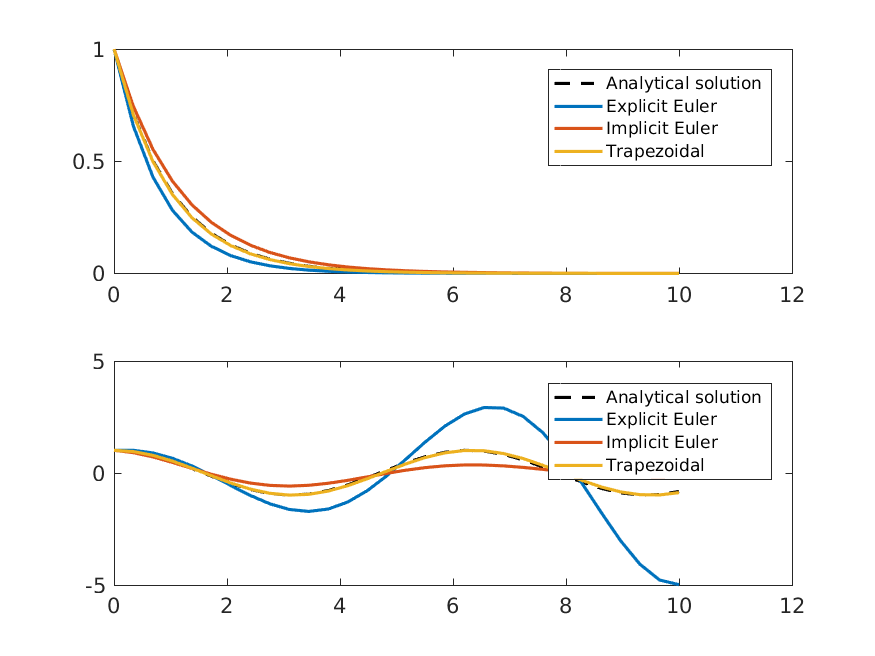
\includegraphics[width=\textwidth]{../Figures/solution1}
    \caption{Explicit, Implicit Euler and Trapezoidal method solution to test equation and harmonic oscillator for h = 0.345}
    \label{fig:sol1}
\end{figure}

All three implimentations of these one step algorithms along with the code for Newton's method can be found in the appendix.

\subsection{Multistep methods}

Even though we see in figure \ref{fig:sol1} that the solution found by the trapezoidal method lies very close to the analytical solution, for some applications one could require higher order approximations to obtain more accurate results.

The classical Runge-Kutta method and its higher order variations play with the concept introduced in last section to create finer approximations to the solution. Concretetly the classical Runge-Kutta method takes four stages to compute a weighted avarage of four different slope estimates. The slope estimation at the fourth stage will be based in the information obtained in the three previous stages.

\begin{equation}\label{eq:ClassicRungeKutta}
\begin{aligned}
T_1 &= t_n &\qquad
X_1 &= x_n \\
T_2 &= t_n + \frac{1}{2} h &
X_2 &= x_n + \frac{1}{2} h f(T_1,X_1) \\
T_3 &= t_n + \frac{1}{2} h &
X_3 &= x_n + \frac{1}{2} h f(T_2,X_2) \\
T_4 &= t_n + h &
X_4 &= x_n + h f(T_3,X_3) \\
t_{n+1} &= t_n + h \span \span \\
x_{n+1} &= x_n + h (\frac{1}{6} f(T_1,X_1) + \frac{1}{2}  f(T_2,X_2) + \frac{1}{2} f(T_3,X_3) + \frac{1}{6} f(T_4,X_4)) \span \span
\end{aligned}
\end{equation}

Equation \ref{eq:ClassicRungeKutta} reveals that since this is an explicit method there is no need for a numerical solver. The coefficients and weights of these equations are often collected in the Butcher's Tableu. This is described more deeply in section 3.

Two different variations of DOPRI54 have also been implemented. DOPRI54 is just another explicit Runge-Kutta method of higher order with more stages and a larger Butcher's Tableu. We shall see when comparing the error estimates the difference between the two methods. The three methods are shown in the appendix.

\subsection{Global and local errors}

It is easy to see in figure \ref{fig:sol1}, especially in the bottom graph, that, since we base the solution at one point on previous approximations, the further the points are from the initial value the more inaccurate they become and the greater the distance to the true solution is. This distance is called global error, whilst the error made in every iteration is known as local error. As we will discuss later the latter is commonly used to classify different methods depending in their accuracy.

\begin{figure}[H]
    \centering
    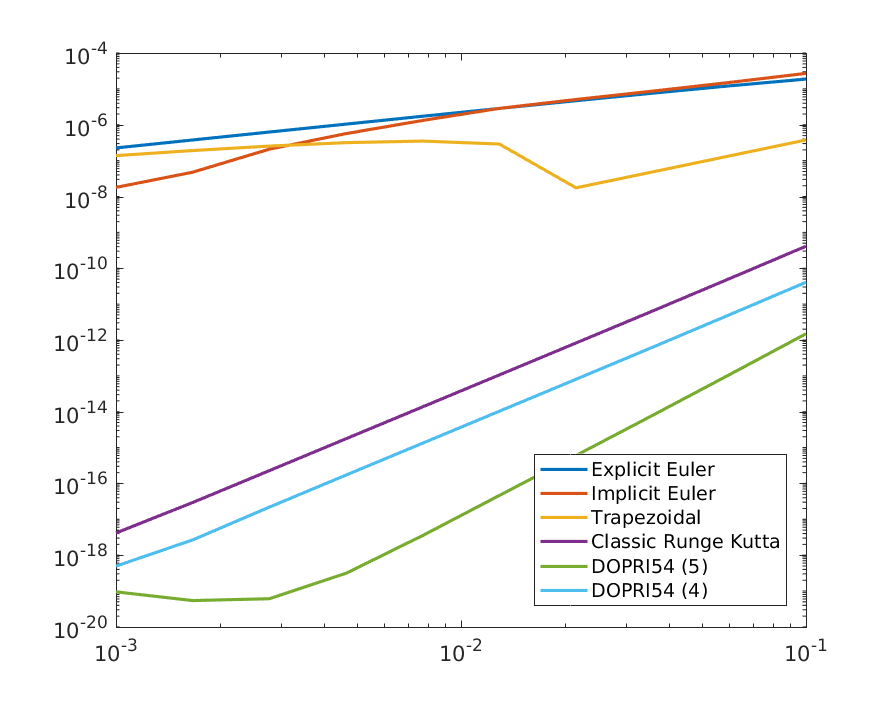
\includegraphics[width=\textwidth]{../Figures/GlobalErrorTest}
    \caption{Explicit, Implicit Euler and Trapezoidal method global errors in test equation}
    \label{fig:global1}
\end{figure}

One could then derive the analytical expression of the solution for both problems and compute te local and global errors.

\begin{equation}
x(t) = \exp(-t) \qquad
x(t) = cos(t)
\end{equation}

\begin{figure}[H]
    \centering
    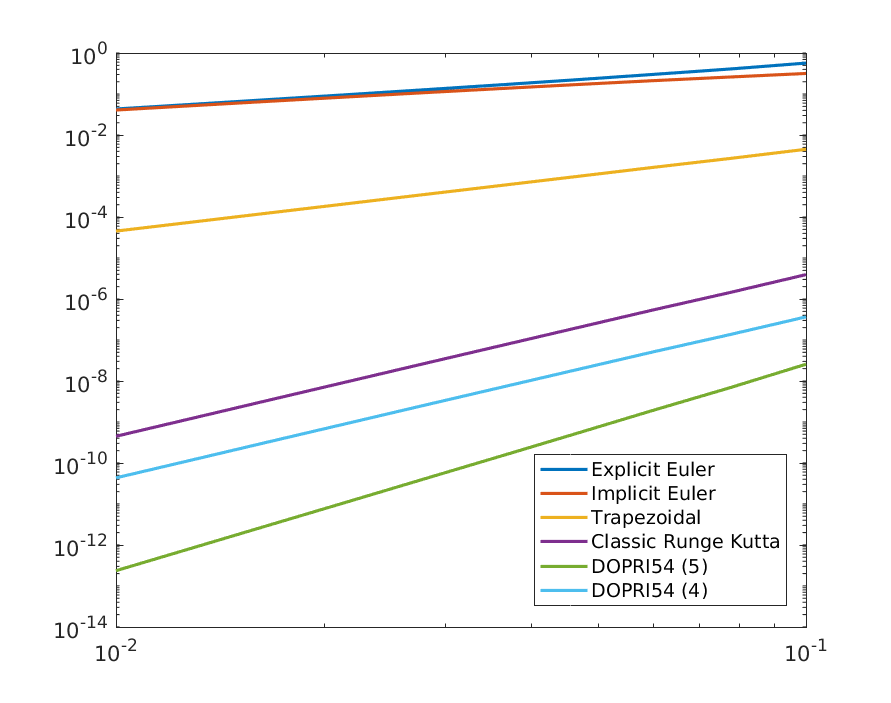
\includegraphics[width=\textwidth]{../Figures/GlobalErrorTest2}
    \caption{Explicit, Implicit Euler and Trapezoidal method global errors in harmonic oscillator}
    \label{fig:global2}
\end{figure}

Figure \ref{fig:global1} represents the global error at time $t = 10$ made by the one step solvers (left graph) and the multistep solver (right graph) for different step sizes. As expected, the size the global error decreases when increasing the number of points used in the approximation.

Why is not good to use global error??

\begin{figure}[H]
    \centering
    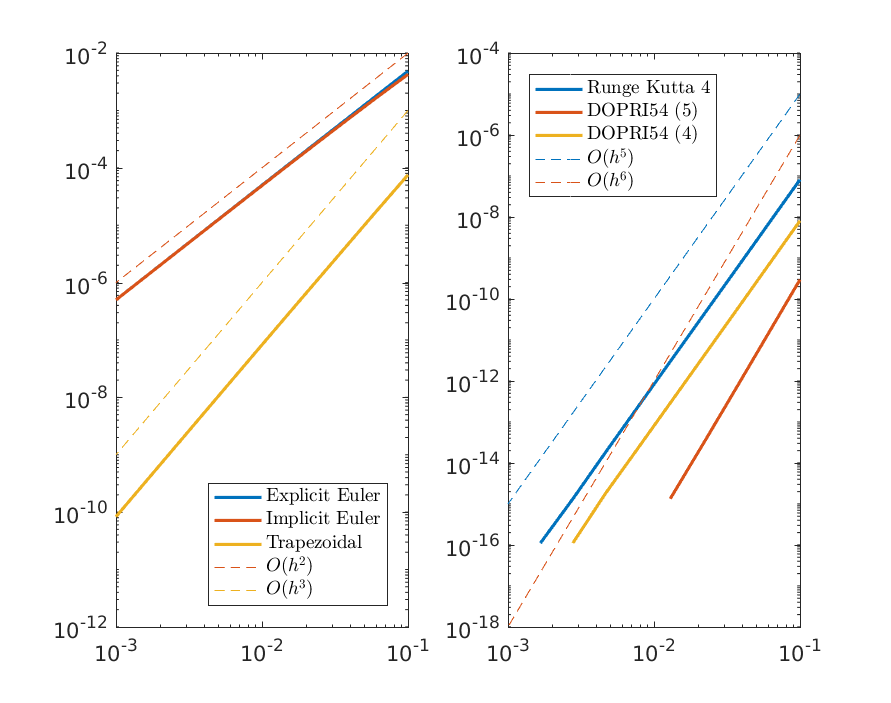
\includegraphics[width=\textwidth]{../Figures/LocalErrorTest1}
    \caption{Explicit, Implicit Euler and Trapezoidal method local errors in test equation}
    \label{fig:LocalErrorTest1}
\end{figure}

On the other hand the local error at time $t = t_0 + h$ is shown in figure \ref{fig:LocalErrorTest1}. Again we see how the error decreases with the step size. Moreover, as the plots use logarithmic scale and the curves are approximately straight lines, we can conclude that there is an exponential dependence between local error and step size or in big O notation: $O(h^{p+1})$. The constant p is used to characterize different methods, thus we say that a method is order 2 when the local error is proportional to$h^{3}$. The dashed lines in figure \ref{fig:local1} can be used to verify the order of the solvers. That is, order 1 for Explicit and Implicit Euler, order 2 for the Trapezoidal method, order 4 for the classical Runge Kutta and one of the DOPRI54 versions and order 5 for the other DOPRI54.

\begin{figure}[H]
    \centering
    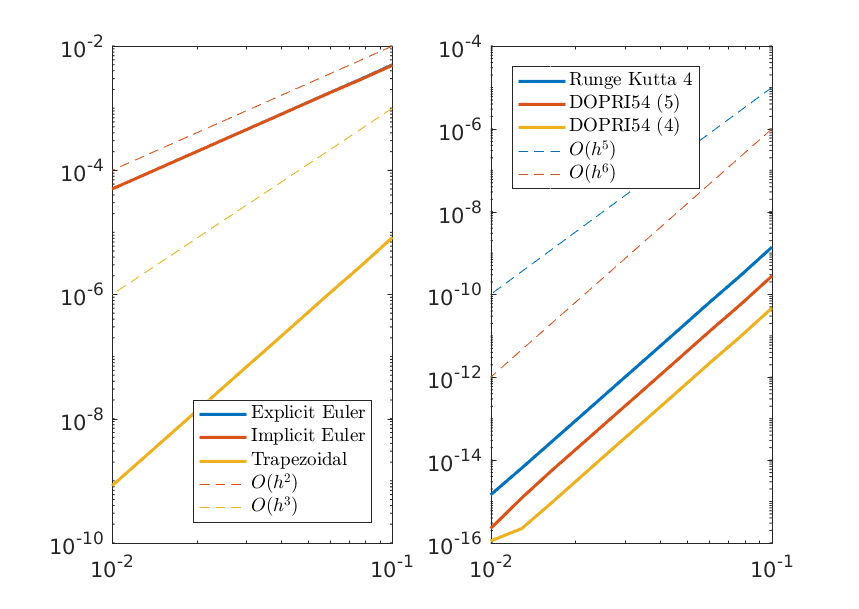
\includegraphics[width=\textwidth]{../Figures/LocalErrorTest2}
    \caption{Explicit, Implicit Euler and Trapezoidal method local errors in harmonic oscillator}
    \label{fig:LocalErrorTest2}
\end{figure}

\subsection{Error estimation}

Considering that the algorithms are used to solve differential equations that are hard to derive analyticaly, calculate the exact error is not always possible.

An easy way to estimate the local error is called step doubling. The solution is computed for ...
(performance). It turns out that estimate is proportional to the exact error and we can then 

More sophisticated algorithms, such as DOPRI54, use embbeded methods of lower order to estimate the error. Even though the estimations obtained as not as good as with step doubling, the secondary method is closely related to the main algorithm so that they can share computations and thus be very efficient. 


\begin{figure}[H]
    \centering
    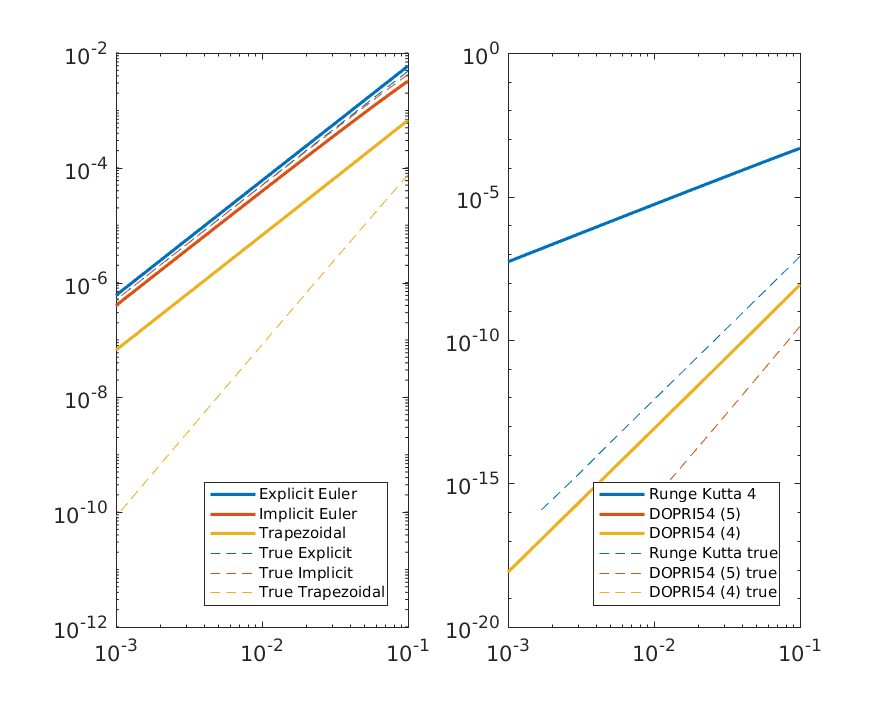
\includegraphics[width=\textwidth]{../Figures/LocalEstimateTest1}
    \caption{Explicit, Implicit Euler and Trapezoidal method local error estimates in test equation}
    \label{fig:Estimate1}
\end{figure}

The local error estimates are plotted along with the true errors in figure \ref{fig:Estimate1} for different step sizes. Even though, they do not match the exact values for some of the methods, the estimates lie always above the true errors which means that they can be used as an upper bound. Besides, as we know that the estimates are proportional to the exact local errors their slope can be used to verify the order of accuracy. In the embedded method estimation the slope is related to the order of lower order algorithm.

\begin{figure}[H]
    \centering
    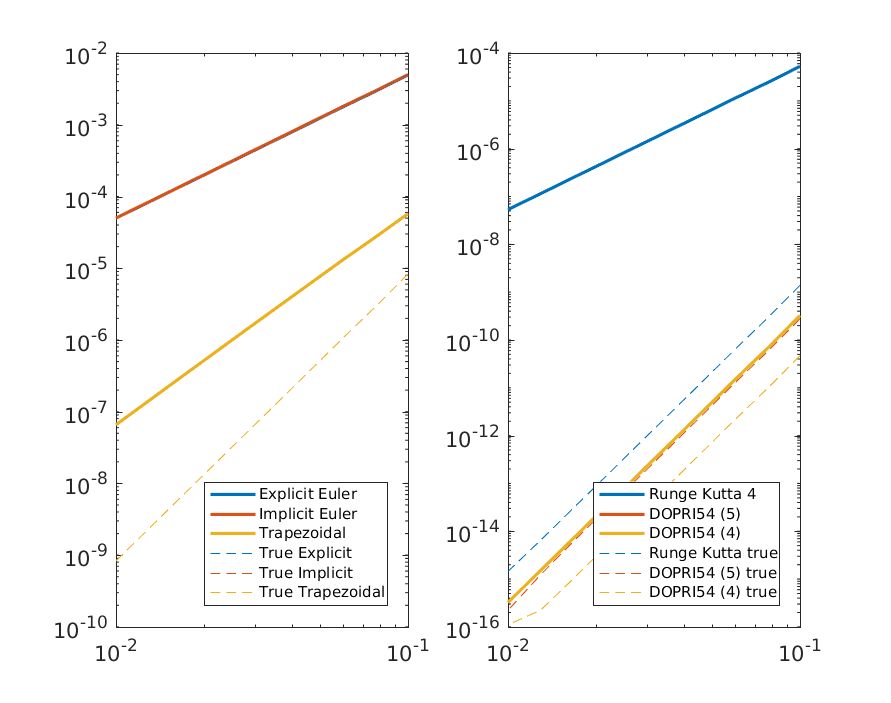
\includegraphics[width=\textwidth]{../Figures/LocalEstimateTest2}
    \caption{Explicit, Implicit Euler and Trapezoidal method local error estimates in harmonic oscillator}
    \label{fig:Estimate2}
\end{figure}